\section{推前积分恒等式}
\label{sec:push-integral-identity}

上一节确定了目标空间上的质量。现在对目标空间上的函数$g$积分：$\int_Yg\,\mathrm d(T_\#\mu)$能否回到原空间计算？直观上，每个点$x$带着质量被送到$T(x)$，在那里读取函数值$g(T(x))$，所以应当有$\int_Yg\,\mathrm d(T_\#\mu)=\int_Xg\circ T\,\mathrm d\mu$。先对指示函数核对。若$g=\mathbf 1_B$，左端是$(T_\#\mu)(B)=\mu(T^{-1}(B))$；而$\mathbf 1_B(T(x))=1$当且仅当$x\in T^{-1}(B)$，即$\mathbf 1_B\circ T=\mathbf 1_{T^{-1}(B)}$，右端也等于$\mu(T^{-1}(B))$。沿积分的构造步骤推广，就得到一般结论。

\begin{theorem}[推前积分恒等式]
\label{thm:push-integral-identity}
设$(X,\mathcal A,\mu)$是测度空间，$T:(X,\mathcal A)\to(Y,\mathcal B)$可测。
\begin{enumerate}
\item 对每个可测$g:Y\to[0,+\infty]$，
\begin{equation}
\int_Yg\,\mathrm d(T_\#\mu)=\int_Xg\circ T\,\mathrm d\mu ,
\label{eq:push-integral-identity}
\end{equation}
两边可以同为$+\infty$。
\item 对可测的实值或复值$g$，$g$关于$T_\#\mu$可积当且仅当$g\circ T$关于$\mu$可积，此时式~\eqref{eq:push-integral-identity}成立且两边有限。
\end{enumerate}
\end{theorem}

\begin{proof}
$g\circ T$是可测映射的复合，因而可测。(1) 指示函数的情形已在上面核对。对非负简单函数$s=\sum_ic_i\mathbf 1_{B_i}$，$s\circ T=\sum_ic_i\mathbf 1_{B_i}\circ T$，两边由线性性相等。对一般非负可测$g$，取非负简单函数$s_n\uparrow g$，则$s_n\circ T\uparrow g\circ T$，两边分别用单调收敛定理取极限。

(2) 由$\lvert g\circ T\rvert=\lvert g\rvert\circ T$，把(1)用于$\lvert g\rvert$，两边的绝对积分相等，可积性等价。实值时$(g\circ T)^\pm=g^\pm\circ T$，对正部和负部分别用(1)后相减，两边都是有限数之差；复值时对实部和虚部分别处理。
\end{proof}

定理只用到可测性与推前测度的定义。它不要求$T$可逆或可微，不要求$X,Y$有距离或坐标，也不要求$T_\#\mu$相对于任何参考测度有密度。这里沿映射转移的是测度，被积函数相应地复合上$T$；这与上一章的换测度公式不同，那里点不移动，被积函数不变，只是累计权重乘上密度。

恒等式可以从两个方向读。已知$\mu$时，它把目标空间上的积分化为原空间上的积分，例如随机变量的函数的期望，可以直接在原来的概率空间上计算，不必先求出输出的分布。反过来，它说明对复合函数$g\circ T$的累计只取决于$T$把质量送到了哪里：两个映射若推前出同一个测度，所有形如$\int g\circ T\,\mathrm d\mu$的积分都相同。

\begin{example}[有限集合上的分组汇总]
\label{ex:push-finite-sum}
取$X=\{1,2,3,4\}$，$\mu(\{k\})=k/10$；$Y=\{0,1\}$，$T(1)=T(3)=1$，$T(2)=T(4)=0$。输出点$0$的原像是$\{2,4\}$，所以$(T_\#\mu)(\{0\})=0.2+0.4=0.6$；同理$(T_\#\mu)(\{1\})=0.1+0.3=0.4$。取$g(0)=5$、$g(1)=2$，左端是$5\times0.6+2\times0.4=3.8$；右端逐个原像点计算$g(T(k))\mu(\{k\})$，得$2\times0.1+5\times0.2+2\times0.3+5\times0.4=3.8$。
\end{example}

图~\ref{fig:push-finite-sum}显示了两种算法的差别：右端逐点累计，左端先把映到同一输出点的质量合并，再乘以该点的函数值。整个计算没有用到任何“输出密度”，输出测度本身就是两个原子。

\begin{figure}[!htbp]
\centering
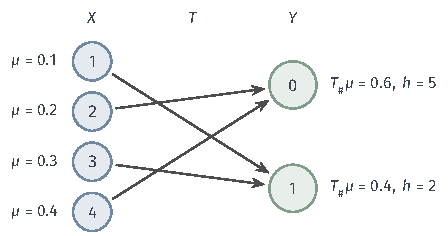
\includegraphics[width=75.812mm]{figures/02-abstract-mathematics/01-metric-and-measure/tikz/c3-pushforward-change/figure.pdf}
\caption{有限集合上的推前与换元。输入点$k=1,2,3,4$的质量为$k/10$，映射$T$把$2,4$送到$0$、把$1,3$送到$1$，输出质量分别为$0.6$与$0.4$。取$h(0)=5$、$h(1)=2$（正文记作$g$），按输出点汇总与按输入点逐个累计都得到$3.8$。}
\label{fig:push-finite-sum}
\end{figure}

\paragraph{连续情形与复合}
在$[0,1]$上取$\mu=\lambda|_{[0,1]}$，$T(x)=\lfloor2x\rfloor$，上一节已求出$T_\#\mu=\tfrac12\delta_0+\tfrac12\delta_1$。对$g(y)=y^2+1$，左端$\tfrac12g(0)+\tfrac12g(1)=\tfrac12+1=\tfrac32$；右端$\int_0^1(\lfloor2x\rfloor^2+1)\,\mathrm dx=\int_0^{1/2}1\,\mathrm dx+\int_{1/2}^12\,\mathrm dx=\tfrac32$，单点$x=1$不影响积分。若接着再作映射$S:Y\to Z$，由$(S\circ T)_\#\mu=S_\#(T_\#\mu)$，式~\eqref{eq:push-integral-identity}可以逐级使用：$\int_Zk\,\mathrm d((S\circ T)_\#\mu)=\int_Yk\circ S\,\mathrm d(T_\#\mu)=\int_Xk\circ S\circ T\,\mathrm d\mu$。

\paragraph{可积性条件}
第2条中的可积性条件不能省。在$(0,1)$上取$\mu=\lambda|_{(0,1)}$，$T(x)=1/x$，把质量送到$(1,\infty)$。对$g(y)=\sin y$，$\int_{(0,1)}\lvert\sin(1/x)\rvert\,\mathrm dx\leq1$，两边都可积，恒等式成立。对$g(y)=y$，$\int_0^1(1/x)\,\mathrm dx=+\infty$，按第1条两边同为$+\infty$，仍是一个正确的等式；但若换成带符号的$g(y)=y\sin y$，可以验证两边的正部与负部积分都是$+\infty$，这时式~\eqref{eq:push-integral-identity}没有意义，而不是不成立。实际使用时，应先对$\lvert g\rvert$用第1条确认可积，再写出有符号的等式。
